\documentclass[a4paper, 12pt]{scrartcl}
\usepackage[polish]{babel}
\usepackage[utf8]{inputenc}
\usepackage[T1]{fontenc}
\usepackage[top=2.5cm, bottom=2.5cm, left=2.5cm, right=2.5cm]{geometry}
\usepackage{enumerate}
\usepackage{hyperref}
\usepackage{graphicx}


\title{Symulacja rozprzestrzeniania się dymu w sali AGH B1 H.24}
\author{Autorzy: Michał Kowalczyk, Kacper Kontny, Denis Lyakhov}
\date{\today}


\begin{document}
	\maketitle
	
	\begin{section}{Cel}
		Głównym założeniem projektu jest stworzenie trójwymiarowego modelu sali wykładowej, a następnie symulacja rozprzestrzeniania się dymu w wyniku wybuchu pożaru w zadanych warunkach. 
	\end{section}
	
	\begin{section}{Narzędzia}
	Symulacja zostanie przeprowadzona przy użyciu silniku FDS (Fire Dynamics Simulator),
    bazującego się na obliczeniu równań różniczkowych (Navier-Stokes).
    
    \vspace{5mm}
    
    Równanie Navier-Stokes’a - w mechanice płynów - równanie różniczkowe cząstkowe,
    opisujące fizykę cieczy. Mówiąc dokładniej, opisuje zmianę prędkości przepływu w czasie.
    Mając aktualny stan prędkości i zbiór sił, równania te mogą nam powiedzieć dokładnie,
    jak zmienia się prędkość w każdym nieskończenie małym przedziale czasu.
    Równania Navier-Stokes’a wyglądają następująco:
    
    \begin{equation}
	    \frac{\partial u}{\partial t} = -(u \cdot \nabla)u+\nu\nabla^{2}u+f
	\end{equation}
	
	\begin{equation}
	    \frac{\partial \rho}{\partial t}=-(u\cdot\nabla)\rho+\kappa\nabla^{2}\rho + S
	\end{equation}

	\end{section}

	\begin{section}{Założenia}
		\begin{enumerate}
			\item Model sali wykładowej wzorowany jest na sali H24 znajdującej się w budynku B1 na terenie kampusu Akademii Górniczo-Hutniczej.
			\item Źródłem dymu jest powierzchnia płaska znajdująca się na podłodze pomiędzy stołem wykładowcy a ławkami uczestników, a więc w najniższym punkcie sali.
			\item Dla uproszczenia symulacji intensywność wydobywania się dymu ze źródła nie zmienia się wraz ze spadkiem zawartości tlenu w badanej atmosferze.
			\item Dla danych scenariuszy zostanie wykonany pomiar temperatury w zadanych punktach przestrzeni.
		\end{enumerate}
	\end{section}

	\begin{section}{Przebieg symulacji}
		Wykonane zostaną symulacje różnych scenariuszy:
		\begin{enumerate}
			\item Źródło dymu niezmienne w czasie, zamknięty obieg powietrza w sali
			\item Źródło dymu ugaszone po pewnym czasie, zamknięty obieg powietrza w sali
			\item Źródło dymu ugaszone po pewnym czasie, otworzenie okien sali w pewnej chwili
			\item Źródło dymu ugaszone po pewnym czasie, włączenie wentylatora oddymiającego w pewnej chwili
		\end{enumerate}
		Symulacja zostanie przeprowadzona przy użyciu programu PyroSim bazującego na silniku FDS (Fire Dynamics Simulator)
	\end{section}

	\begin{section}{Wyniki symulacji}
		\begin{subsection}{Źródło dymu niezmienne w czasie, zamknięty obieg powietrza w sali}
			\begin{enumerate}[i]
				\item Wykres pomiarów średniej temperatury panującej w pomieszczeniu w funkcji czasu: \\
				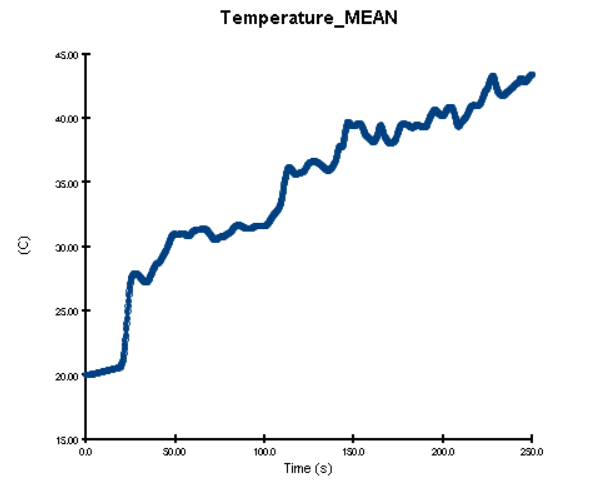
\includegraphics{../H24_Constant_Smoke/temperature} \newpage
				\item Wykres pomiarów średniej widoczności panującej w pomieszczeniu w funkcji czasu:
				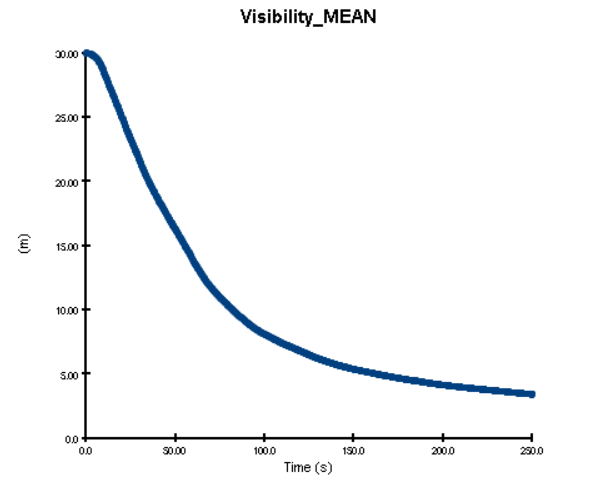
\includegraphics{../H24_Constant_Smoke/visibility}
			\end{enumerate}
		\end{subsection}
		
		\begin{subsection}{Źródło dymu ugaszone po pewnym czasie, zamknięty obieg powietrza w sali}
			\begin{enumerate}[i]
				\item Wykres pomiarów średniej temperatury panującej w pomieszczeniu w funkcji czasu: \\
				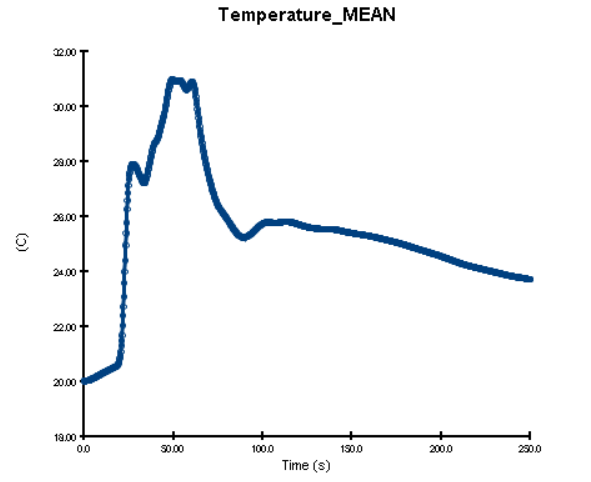
\includegraphics{../H24_Finite_Smoke/temp} \newpage
				\item Wykres pomiarów średniej widoczności panującej w pomieszczeniu w funkcji czasu:
				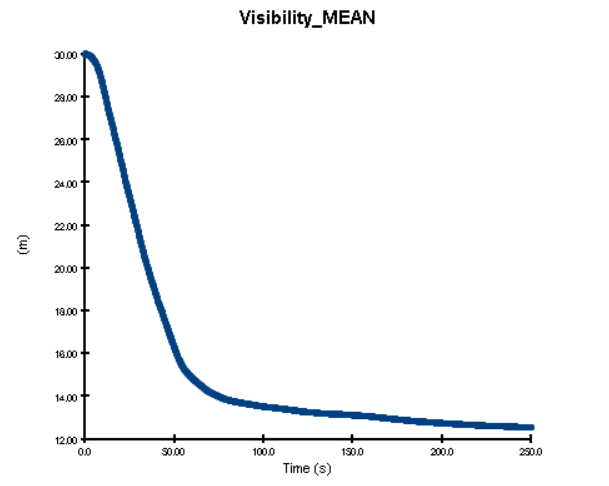
\includegraphics{../H24_Finite_Smoke/visibility}
			\end{enumerate}
		\end{subsection}
	
		\begin{subsection}{Źródło dymu ugaszone po pewnym czasie, otworzenie okien sali w pewnej chwili}
			\begin{enumerate}[i]
				\item Wykres pomiarów średniej temperatury panującej w pomieszczeniu w funkcji czasu: \\
				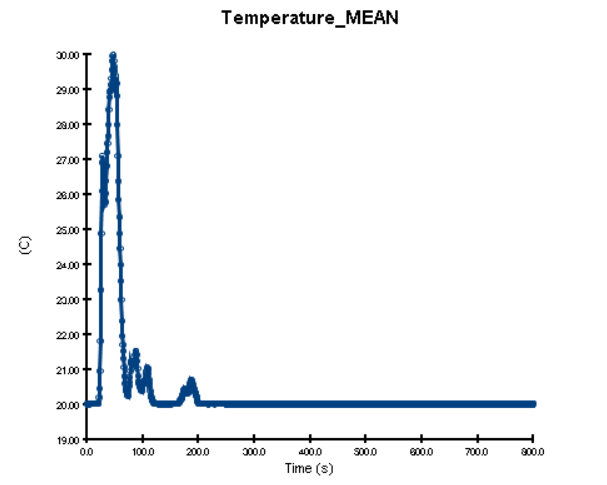
\includegraphics{../H24_Windows/temp} \newpage
				\item Wykres pomiarów średniej widoczności panującej w pomieszczeniu w funkcji czasu:
				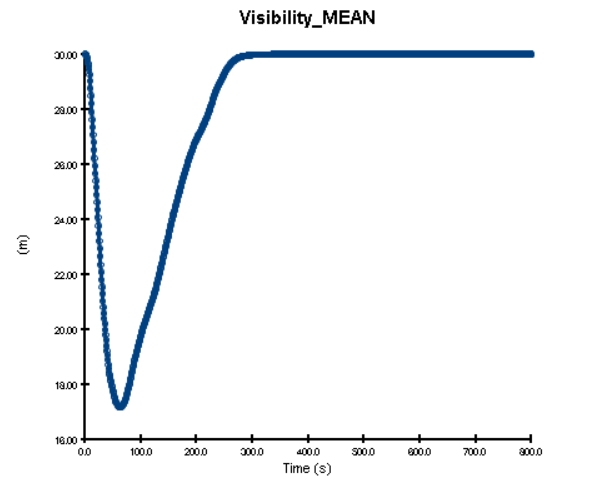
\includegraphics{../H24_Windows/visibility}
			\end{enumerate}
		\end{subsection}
		
		\begin{subsection}{Źródło dymu ugaszone po pewnym czasie, włączenie wentylatora oddymiającego w pewnej chwili}
			\begin{enumerate}[i]
				\item Wykres pomiarów średniej temperatury panującej w pomieszczeniu w funkcji czasu: \\
				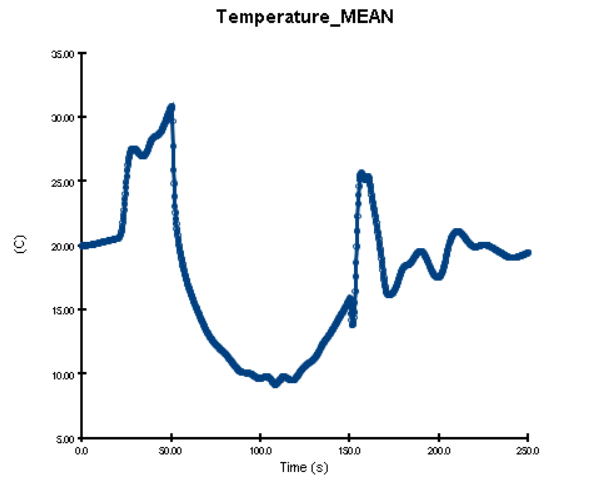
\includegraphics{../H24_Ventilation/temperature} \newpage
				\item Wykres pomiarów średniej widoczności panującej w pomieszczeniu w funkcji czasu:
				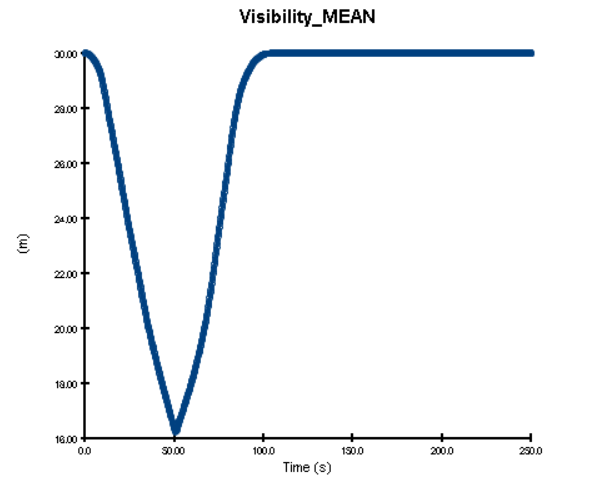
\includegraphics{../H24_Ventilation/visibility}
			\end{enumerate}
		\end{subsection}
		
	\end{section}
	
	\begin{section}{Opracowanie wyników i wnioski}
		\begin{enumerate}
			\item Pierwsze dwie symulacje są symulacjami referencyjnymi - pozwalają ocenić jak w przypadku niewykrytego pożaru mógłby rozprzestrzeniać się dym w sali. Jak widać na załączonych wykresach, jeżeli dym nie zostanie ugaszony, średnia temperatura całego pomieszczenia będzie nierównomiernie, lecz sukcesywnie rosnąć. \\
			W przypadku ugaszenia źródła dymu temperatura pomieszczenia zaczyna powoli wracać do normy, lecz ogólne zadymienie pomieszczenia nie zmniejsza się - średnia widoczność nadal maleje, ale zdecydowanie wolniej.
			\item Trzecia symulacja zakładała otwarcie okien zaraz po całkowitym zgaszeniu źródła dymu, żeby nie doprowadzić do podsycenia ognia tlenem. Założyliśmy iż w pomieszczeniu znajdują się cztery automatycznie otwierane okna o powierzchni $ 1m^2 $ każde, co daje łącznie $ 4m^2 $ powierzchni czynnej. \\
			Czynności przeciwpożarowe i oddymiające zostały wdrożone w 40. sekundzie symulacji. Średnia temperatura sali powróciła do normy w ok. 200 sekundzie, a widoczność w 250. Temperatura ustabilizowała się więc ok. 160 sekund po otwarciu okien, a widoczność po 210.
			\item Czwarta symulacja zakładała uruchomienie wentylatorów oddymiających w sytuacji podobnej do symulacji z otwarciem okien. Dla łatwego porównania zastosowaliśmy również cztery wentylatory o łącznej powierzchni $ 4m^2 $ i przepustowości całkowitej $ 72000 m^3/h $. \\
			Czynności przeciwpożarowe i oddymiające zostały wdrożone w 50. sekundzie symulacji. Średnia temperatura sali powróciła do normy w ok. 2500 sekundzie, a widoczność w 90. Temperatura ustabilizowała się więc ok. 2450 sekund po otwarciu okien, a widoczność po 40.
		\end{enumerate}
		\textbf{WNIOSKI}
		\begin{enumerate}
			\item Brak systemu przeciwpożarowego i oddymiającego ze względu na sposób i prędkość rozprzestrzeniania się dymu mogą prowadzić do groźnych konsekwencji nawet dla osób znajdujących się z dala od źródła dymu.
			\item Samo zlikwidowanie źródła dymu nie gwarantuje usunięcia zagrożenia, ponieważ nieodprowadzony dym będzie zalegał w sali, wymagana jest w takim przypadku ewakuacja i jak najszybsza wentylacja pomieszczenia.
			\item W sytuacji, w której po zgaszeniu źródła dymu samoistnie zostaną otworzone okna, dym w bezpieczny sposób będzie odprowadzany, lecz wydajność tego systemu może być w pewnych przypadkach niewystarczająca; jeśli źródło dymu będzie dość duże, a sala pełna ludzi, może dojść do paniki która spowolni ewakuację, a co za tym idzie ryzyko negatywnego wpływu dymu na organizm drastycznie wzrasta.
			\item Włączenie wentylatorów oddymiających zdecydowanie przyspieszało proces oczyszczania powietrza sali, pomimo iż pomieszczenie zadymiało się dłużej, jego wietrzenie trwało zdecydowanie krócej.
			\item Prędkość z jaką wentyluje się pomieszczenie jest bezpośrednio związane z wydajnością systemu oddymiającego - okna jedynie pozwalają na wymianę powietrza przez różnicę ciśnień wywołaną różnicą temperatur, a wentylatory wyciągają zanieczyszczone powietrze z sali, co czyni ten sposób efektywniejszym.
			\item Pomiary temperatury średniej panującej w pomieszczeniu przy użyciu wentylatorów zmienia się nieregularnie - po drastycznym spadku zaczyna rosnąć, a następnie ponownie maleć. Dzieje się tak ze względu na nagła zmianę ciśnień w pomieszczeniu, wskazania temperatury po wzroście są jednak zdecydowanie mniejsze niż najwyższe, przy aktywnym źródle ognia, co nie wprowadza niepożądanych skutków.
			
		\end{enumerate}
		
	\end{section}

	\begin{section}{Źródła}
		
		PyroSim Fire Dynamics and Smoke Control by Thunderhead Engineering Consultants, Inc. \textit{\href{https://www.thunderheadeng.com/pyrosim/}{link}}.
		\begin{thebibliography}{15}
			\bibitem{id}
				Eren Algan, \textit{REAL-TIME SMOKE SIMULATION},
				\textit{\href{http://repository.bilkent.edu.tr/bitstream/handle/11693/15609/0006332.pdf?sequence=1&isAllowed=y}{link}}.
				
			\bibitem{id2}
				Jos Stam, \textit{Real-Time Fluid Dynamics for Games}.
				
			\bibitem{id3}
				Marinus Rorbech, \textit{REAL-TIME SIMULATION OF SMOKE USING GRAPHICS HARDWARE},
				\textit{\href{http://image.diku.dk/projects/media/roerbech.04.pdf}{link}}.
		\end{thebibliography}
	\end{section}
	
	

\end{document}